% !TEX root=meca1321-synthesis.tex

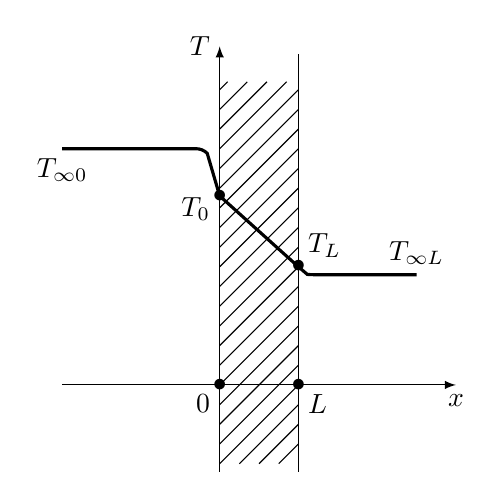
\begin{tikzpicture}
  \draw [>=latex, ->] (-2, 0) -- (3, 0) node [below] {$x$};
  \draw [>=latex, ->] (0, -1.1) -- (0, 4.3) node [left] {$T$};
  \draw (0, 0) node {$\bullet$};
  \draw (0, 0) node [below left] {$0$};
  \draw (1, 0) node {$\bullet$};
  \draw (1, 0) node [below right] {$L$};
  \draw (1, -1.1) -- (1, 4.2);
  \foreach \i in {-4, ..., 11}
  {
    \pgfmathsetmacro{\x}{(\i/4)};
    \draw (0, \x) -- ++(1, 1);
  }
  \draw (0.25, -1) -- ++(0.75, 0.75);
  \draw (0.50, -1) -- ++(0.5, 0.5);
  \draw (0.75, -1) -- ++(0.25, 0.25);
  \draw (0, 3) -- ++(0.85, 0.85);
  \draw (0, 3.25) -- ++(0.6, 0.6);
  \draw (0, 3.5) -- ++(0.35, 0.35);
  \draw (0, 3.75) -- ++(0.1, 0.1);
  \draw (0, 2.4) node {$\bullet$};
  \draw (1, 1.5) node {$\bullet$};
  \draw [line width = 0.4mm] (1, 1.5) -- (0, 2.4);
  \draw (0, 2.5) node [below left] {$T_0$};
  \draw (1, 1.5) node [above right] {$T_L$};

  \draw [line width = 0.4mm] (-2, 3) -- (-0.3, 3) arc (90:45:0.2) -- (0, 2.4);
  \draw (-2, 3) node [below] {$T_{\infty 0}$};
  \draw [line width = 0.4mm] (2.5, 1.4) -- (1.2, 1.4) arc (270:265:1) -- (1,1.5);
  \draw (2.5, 1.4) node [above] {$T_{\infty L}$};
\end{tikzpicture}
